\section{Вывод уравнения струны}
Пусть есть струна, закрепленная в точках $0, l$. И мы эту струну оттягиваем от положения равновесия:

\begin{figure}[H]
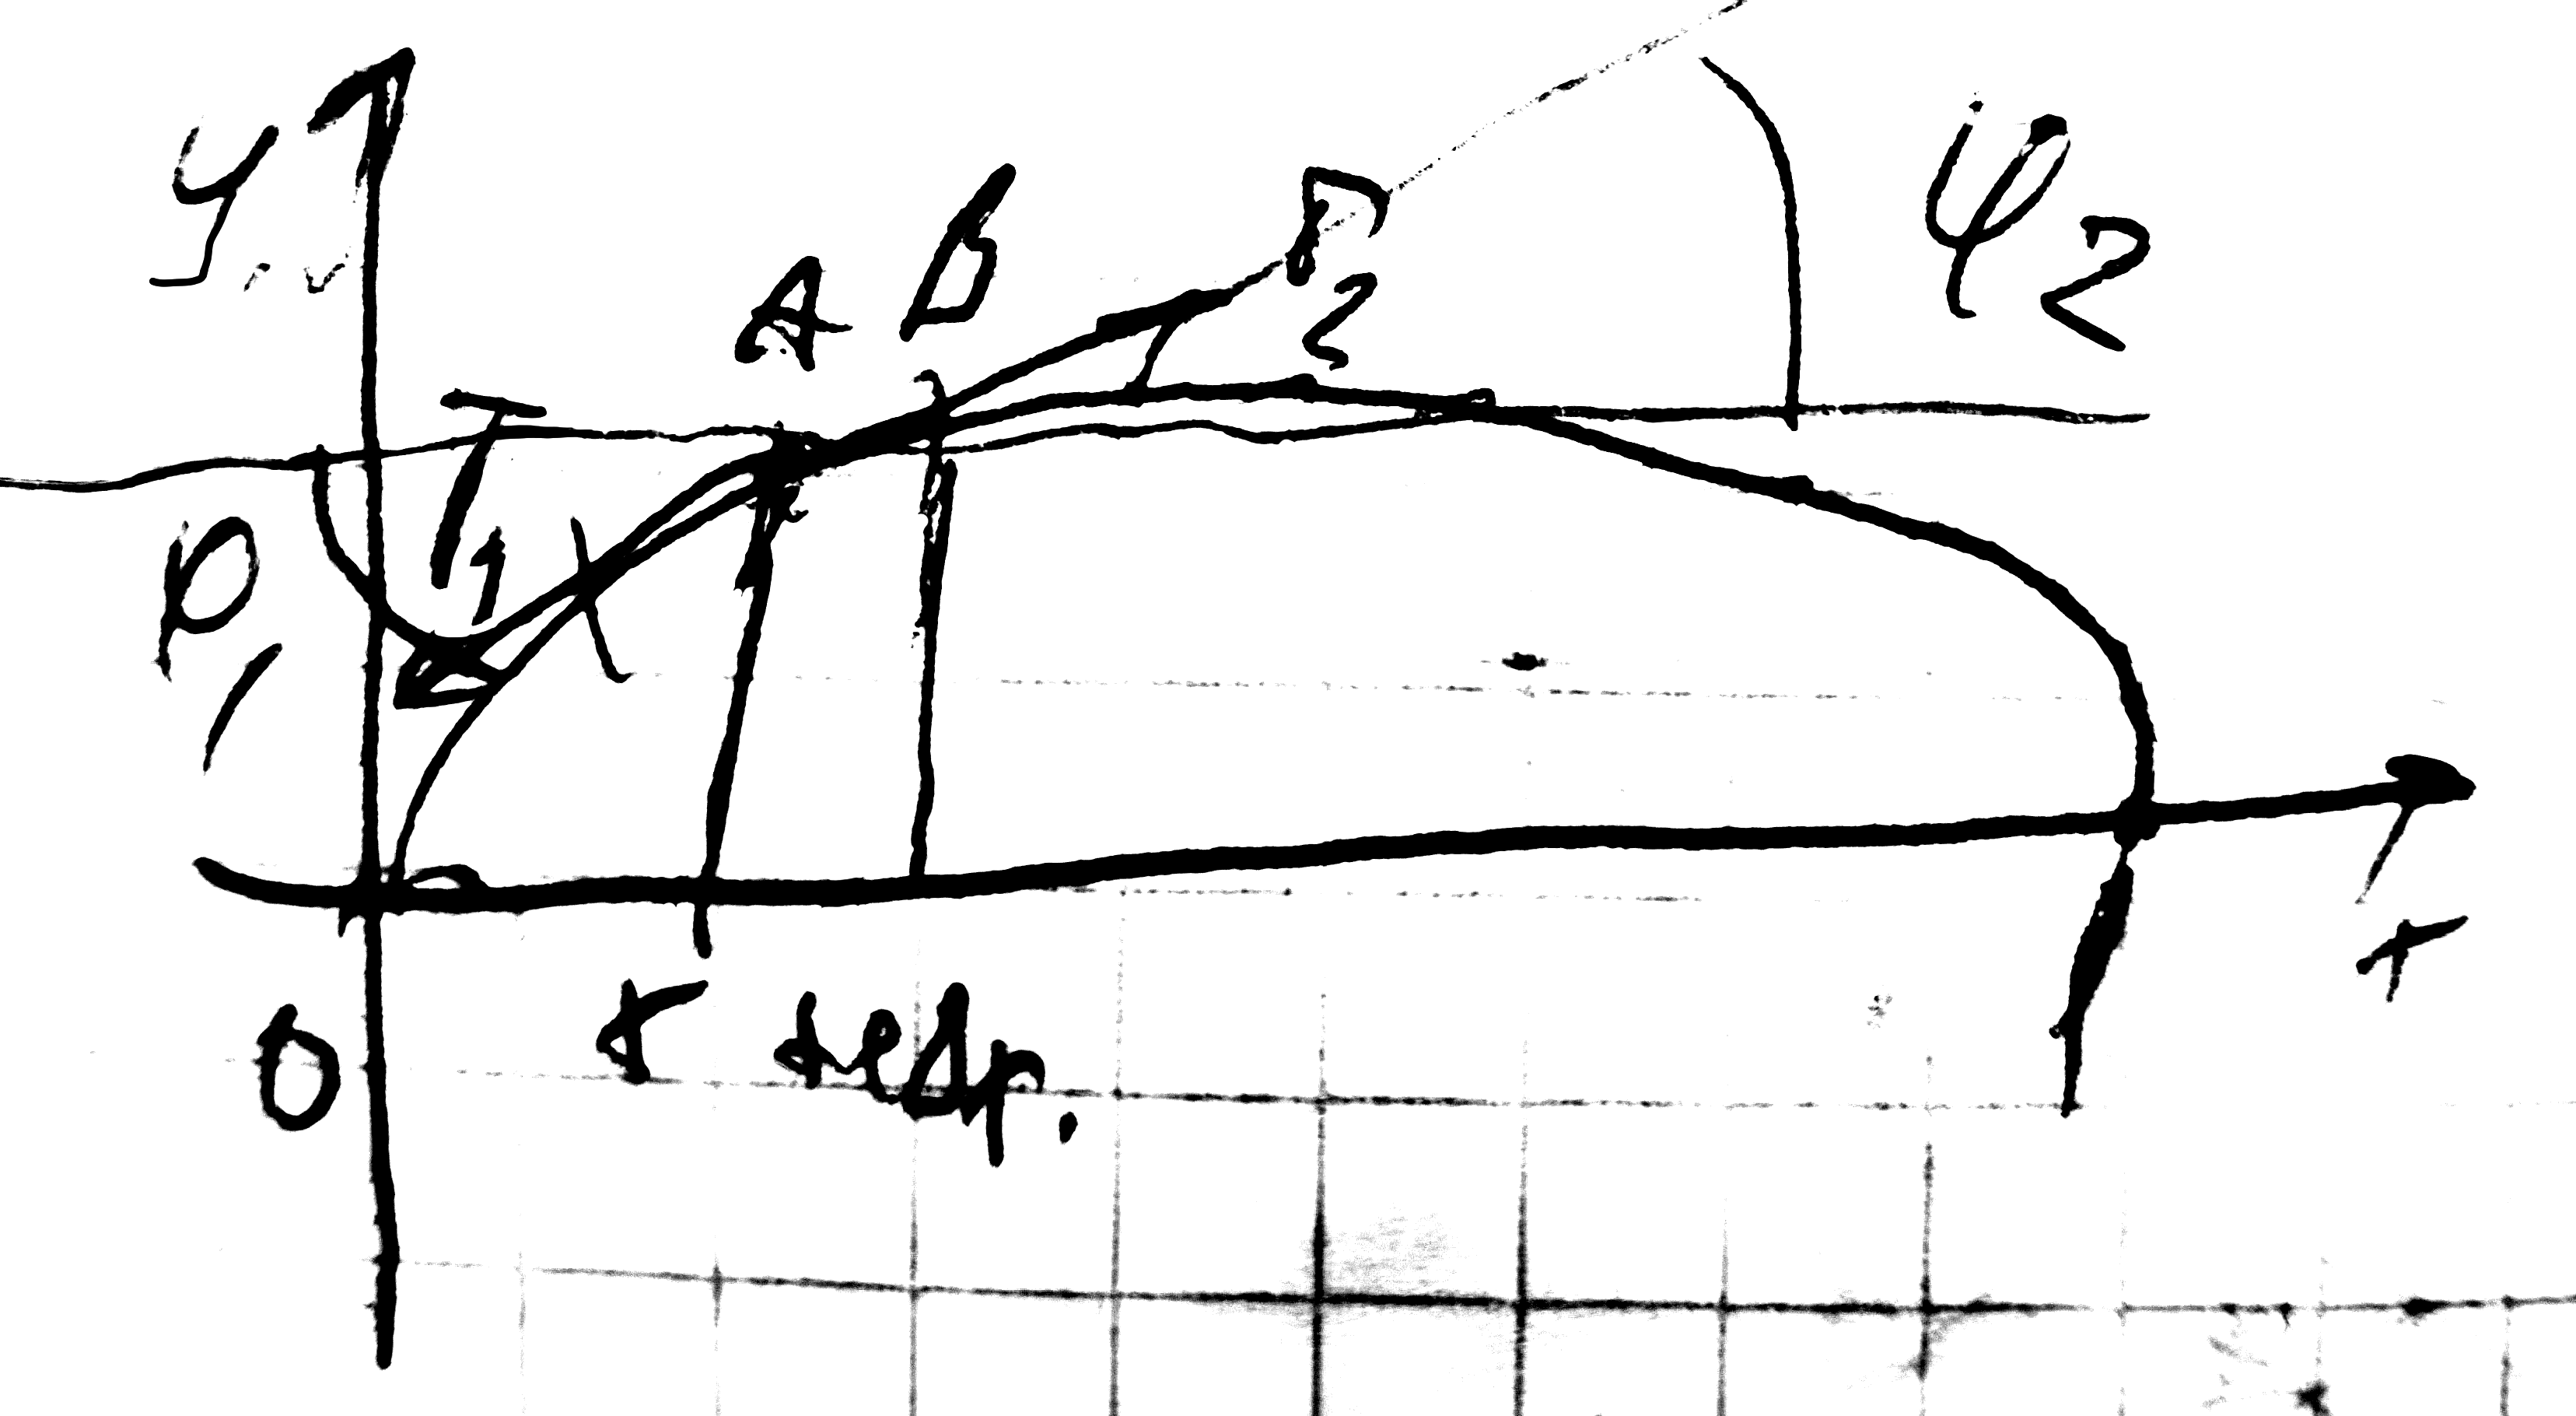
\includegraphics[width=\textwidth]{1}
\end{figure}

Силой тяжести мы пренебрегаем, продольное движение отсутствует, а остаются только две силы натяжения нити $T_1, T_2$. Спроецируем их на оси:
\[
		Ox: 0=-T_1 \cos \varphi_1 + T_2 \cos \varphi_2
\]
\[
	\begin{aligned}
		\sin \varphi = \frac{\frac{\partial u}{\partial x}}{\sqrt{1 + \left( \frac{\partial u}{\partial x}\right)^2}} \approx \frac{\partial u}{\partial x}\\
	\cos \varphi = \frac{1}{\sqrt{1 + \left( \frac{\partial u}{\partial x}\right)^2}} \approx 1
\end{aligned}
\]
Отсюда получается, что $T_1 \approx T_2 =: T$. Спроецируем на $Ou:$
\[
	\begin{aligned}
	ma = T \sin\varphi_2 - T \sin \varphi_1 \\
	ma = T \left(\left. \frac{\partial u}{\partial x}\right|_{x = x+\Delta x} - \left. \frac{\partial u}{\partial x}\right|_{x=x} \right)
\end{aligned}
\]
Массу можно представить в виде $m = l \cdot \rho$, где $l$ - длина, $\rho=const$ - линейная плотность, тогда
\[
	l = \int\limits_{AB} ds = \int\limits_x^{x+\Delta x} \sqrt{1 + \left( \frac{\partial u}{\partial x}\right)^2}dx \approx \Delta x
\]
Отсюда
\[
	\begin{aligned}
	m = \rho \cdot \Delta x \\
	\rho \Delta x \frac{\partial^2 u}{\partial t^2} = T \left(\left. \frac{\partial u}{\partial x}\right|_{x = x+\Delta x} - \left. \frac{\partial u}{\partial x}\right|_{x=x} \right) \\
			\rho \frac{\partial^2u}{\partial t^2} = T \frac{\partial^2 u}{\partial x^2} \\
			\frac{\partial^2 u}{\partial t^2} = a^2 \frac{\partial^2 u}{\partial x^2}
		\end{aligned}
\]
Уравнения в частных производных отличаются от обыкновенных дифференциальных уравнений тем, что в обыкновенных диффурах конечное число степеней свободы, а в уравнениях в частной производной - бесконечно много.
